\chapter{Non-premixed (diffusion) flames}
\label{ch:nonpremixed}

In a non-premixed flame fuel and oxidiser arrive \emph{separately} and must mix by diffusion before
they can burn: candle, diesel spray, most industrial burners, rocket engines. The flame cannot
propagate into either stream alone. It sits where the two meet in the right proportion.
Project Part~2 is about this situation.

\section{Configurations}

\begin{figure}[H]
\centering
\begin{tikzpicture}
  % jet flame
  \begin{scope}
    \draw[thick] (-0.25,-1.6) -- (-0.25,0); \draw[thick] (0.25,-1.6) -- (0.25,0);
    \draw[very thick,hot] (-0.25,0) .. controls (-0.9,1.4) and (-0.4,2.8) .. (0,3.2)
                         .. controls (0.4,2.8) and (0.9,1.4) .. (0.25,0);
    \draw[flow] (0,-1.4) -- (0,-0.2);
    \node[lbl,cold] at (0.75,-1.0) {fuel};
    \draw[flow] (-1.6,0.8) -- (-0.8,0.8) node[pos=0,left,lbl] {air};
    \draw[flow] (1.6,0.8) -- (0.8,0.8);
    \node[lbl,align=center] at (0,-2.1) {jet diffusion flame};
  \end{scope}
  % counterflow
  \begin{scope}[xshift=6.5cm,yshift=0.8cm]
    \fill[gray!30] (-1.2,1.6) rectangle (1.2,2.0); \fill[gray!30] (-1.2,-1.6) rectangle (1.2,-2.0);
    \node[lbl] at (0,2.3) {fuel nozzle}; \node[lbl] at (0,-2.3) {oxidiser nozzle};
    \foreach \s in {-1,1} {
      \draw[cold,thick,->] (0.15*\s,1.55) .. controls (0.2*\s,0.4) .. (1.9*\s,0.15);
      \draw[cold,thick,->] (0.6*\s,1.55) .. controls (0.7*\s,0.8) .. (1.9*\s,0.55);
      \draw[cold,thick,->] (0.15*\s,-1.55) .. controls (0.2*\s,-0.4) .. (1.9*\s,-0.15);
      \draw[cold,thick,->] (0.6*\s,-1.55) .. controls (0.7*\s,-0.8) .. (1.9*\s,-0.55);
    }
    \draw[dashed] (-2,0) -- (2,0) node[right,lbl] {stagnation plane};
    \draw[very thick,hot] (-1.8,-0.35) -- (1.8,-0.35) node[right,lbl] {flame};
    \draw[->] (-2.6,-1.4) -- (-2.6,1.4) node[above,lbl] {$x$};
  \end{scope}
\end{tikzpicture}
\caption{Left: jet flame (complex 2D geometry). Right: \textbf{counterflow} flame. Opposed jets create a
stagnation plane. The flame sits on the oxidiser side (for most fuels $\Zst$ is small) where the
mixture is stoichiometric. Along the centreline the problem is exactly one-dimensional, which is
why Cantera can solve it with detailed chemistry.}
\label{fig:cfgeom}
\end{figure}

\section{The mixture fraction}
\label{sec:Z}

\begin{derivation}[a conserved scalar from two reacting ones]
Model the chemistry as one step on a mass basis, $1\,\text{kg F}+s\,\text{kg O}\to(1+s)\,\text{kg P}$,
where $s$ is the \textbf{stoichiometric oxygen-to-fuel mass ratio}. With equal diffusivities $D$
and writing $\mathcal L(\cdot)=\partial_t(\rho\,\cdot)+\divg(\rho\vu\,\cdot)-\divg(\rho D\nabla\,\cdot)$:
\[
\mathcal L(Y_F)=W_F\wdot_F,\qquad \mathcal L(Y_O)=s\,W_F\wdot_F .
\]
The combination $\beta=sY_F-Y_O$ satisfies $\mathcal L(\beta)=0$: \textbf{no source}. Normalise it so
that it is 1 in the fuel stream (1) and 0 in the oxidiser stream (2):
\begin{equation}
  Z=\frac{sY_F-Y_O+Y_{O,2}}{sY_{F,1}+Y_{O,2}} .
  \label{eq:Zdef}
\end{equation}
$Z$ is the mass fraction of material that originated in the fuel stream. It is conserved
(convected and diffused but never created or destroyed), no matter how the chemistry proceeds.
\end{derivation}
\begin{symbols}
$s$ & stoichiometric oxygen-to-fuel mass ratio (kg O per kg F) & \nodim\\
$Y_F$, $Y_O$ & fuel, oxidiser mass fraction & \nodim\\
$D$ & common diffusivity & \si{\metre\squared\per\second}\\
$\mathcal L(\cdot)$ & transport operator (unsteady + convection $-$ diffusion) & \si{\kilo\gram\per\metre\cubed\per\second} $\times$ unit of argument\\
$W_F\wdot_F$ & fuel mass production rate & \si{\kilo\gram\per\metre\cubed\per\second}\\
$\beta=sY_F-Y_O$ & coupling function (conserved) & \nodim\\
$Y_{F,1}$, $Y_{O,2}$ & fuel mass fraction in stream 1 (fuel), oxygen in stream 2 (oxidiser) & \nodim\\
$Z$ & mixture fraction & \nodim\\
\end{symbols}

\begin{derivation}[stoichiometric mixture fraction]
Stoichiometric means fuel and oxygen in exactly the ratio $1:s$, i.e.\ $sY_F=Y_O$. Then $\beta=0$ and
\begin{equation}
  \Zst=\frac{Y_{O,2}}{sY_{F,1}+Y_{O,2}}=\frac{1}{1+sY_{F,1}/Y_{O,2}} .
  \label{eq:Zst}
\end{equation}
\textbf{Methane/air:} $\ce{CH_4}+2\ce{O_2}$, so $s=2\cdot32/16=4$; $Y_{F,1}=1$, $Y_{O,2}=0.233$:
$\Zst=1/(1+4/0.233)=0.055$. This matches Cantera's \code{gas.mixture\_fraction(...)} ($0.0552$).
\end{derivation}
\begin{symbols}
$\Zst$ & stoichiometric mixture fraction & \nodim\\
$s$ & stoichiometric O-to-F mass ratio, $\nu_{O_2}W_{O_2}/W_F$ & \nodim\\
$Y_{F,1}$, $Y_{O,2}$ & fuel in fuel stream, oxygen in air ($0.233$) & \nodim\\
32, 16 & molar masses of \ce{O_2} and \ce{CH_4} & \si{\kilo\gram\per\kilo\mole}\\
\end{symbols}

\begin{warning}[$\Zst$ formula with air]
If you see $\Zst=1/(1+\nu W_F/W_{O_2})$-type expressions, check what $\nu$ means and whether the
oxidiser is pure \ce{O_2} or air. With air you \emph{must} include $Y_{O_2,\rm air}=0.233$ as in
\eqref{eq:Zst}. A useful check: $\Zst$ equals the fuel mass fraction of the stoichiometric
\emph{premixed} mixture (compare the \ce{H_2} example in \secref{sec:composition}).
\end{warning}

\paragraph{Bilger's definition.} With detailed chemistry ``fuel'' and ``oxygen'' are spread over many
species. Bilger defines $Z$ from \emph{element} mass fractions, which only diffusion can change:
\begin{equation}
  Z=\frac{\beta-\beta_2}{\beta_1-\beta_2},\qquad
  \beta=2\frac{Y_C}{W_C}+\frac12\frac{Y_H}{W_H}-\frac{Y_O}{W_O},
\end{equation}

\begin{symbols}
$Y_C$, $Y_H$, $Y_O$ & elemental mass fractions of C, H, O & \nodim\\
$W_C$, $W_H$, $W_O$ & atomic molar masses (12, 1.008, 16) & \si{\kilo\gram\per\kilo\mole}\\
$\beta$, $\beta_1$, $\beta_2$ & Bilger coupling function (local, fuel stream, oxidiser stream) & \si{\kilo\mole\per\kilo\gram}\\
\end{symbols}
where the coefficients count how much oxygen each element needs. Cantera:
\code{gas.mixture\_fraction(fuel, oxidizer, element="Bilger")} or
\code{flame.mixture\_fraction("Bilger")}.

\begin{derivation}[$Z\leftrightarrow\phi$]
Before reaction, a mixture with mixture fraction $Z$ has $Y_F=ZY_{F,1}$ and $Y_O=(1-Z)Y_{O,2}$. Its
equivalence ratio is $\phi=(Y_F/Y_O)/(Y_F/Y_O)_{\rm st}$, so
\begin{equation}
  \phi=\frac{Z}{1-Z}\cdot\frac{1-\Zst}{\Zst},\qquad Z=\frac{\phi\Zst}{1-\Zst+\phi\Zst}.
\end{equation}
Every point in a non-premixed flame is a premixed mixture of some local $\phi$, from $0$ (air)
to $\infty$ (pure fuel).
\end{derivation}
\begin{symbols}
$\phi$ & local equivalence ratio of the unreacted mixture & \nodim\\
$Z$, $\Zst$ & mixture fraction, stoichiometric value & \nodim\\
$Y_F$, $Y_O$ & fuel, oxygen mass fraction before reaction & \nodim\\
\end{symbols}

\section{Infinitely fast chemistry: Burke--Schumann}
\label{sec:BS}

If chemistry is infinitely fast and complete, fuel and oxygen cannot coexist. Lean of $\Zst$ there is no
fuel; rich of it, no oxygen. Since $Y_F$, $Y_O$ (and, with $\mathrm{Le}=1$ and constant $c_p$, $T$)
are then linear in $Z$ on each side:
\begin{align}
  Z\le\Zst:&\quad Y_F=0,\quad Y_O=Y_{O,2}\Big(1-\frac Z{\Zst}\Big),\quad
  T=T_2+Z(T_1-T_2)+\frac{QY_{F,1}}{c_p}Z,\\
  Z\ge\Zst:&\quad Y_O=0,\quad Y_F=Y_{F,1}\frac{Z-\Zst}{1-\Zst},\quad
  T=T_2+Z(T_1-T_2)+\frac{QY_{F,1}}{c_p}\Zst\frac{1-Z}{1-\Zst}.
\end{align}

\begin{symbols}
$Q$ & heat of combustion per kg of fuel & \si{\joule\per\kilo\gram}\\
$c_p$ & specific heat capacity (assumed constant) & \si{\joule\per\kilo\gram\per\kelvin}\\
$T_1$, $T_2$ & fuel-stream, oxidiser-stream temperatures & \si{\kelvin}\\
$Y_F$, $Y_O$, $Z$ & fuel and oxidiser mass fractions, mixture fraction & \nodim\\
\end{symbols}

\begin{figure}[H]
\centering
\begin{tikzpicture}[xscale=6,yscale=1.4]
  \draw[->] (0,0) -- (1.05,0) node[right] {$Z$};
  \draw[->] (0,0) -- (0,3.4);
  \draw[very thick,hot] (0,0.3) -- (0.1,3.0) -- (1,0.3);
  \draw[very thick,hot,dashed] (0,0.3) .. controls (0.07,2.4) and (0.09,2.65) .. (0.1,2.7) .. controls (0.16,2.2) and (0.4,1.0) .. (1,0.3);
  \draw[thick,cold] (0,2.4) -- (0.1,0);
  \node[cold,lbl,left] at (0,2.4) {$Y_{O,2}$};
  \node[cold,lbl] at (0.13,0.45) {$Y_O$};
  \draw[thick,keyc] (0.1,0) -- (1,2.4);
  \node[keyc,lbl,right] at (1,2.4) {$Y_F\to Y_{F,1}$};
  \draw[dotted] (0.1,0) -- (0.1,3.1);
  \node[lbl,below] at (0.1,0) {$\Zst$};
  \node[hot,lbl,anchor=west] at (0.2,3.15) {$T$: Burke--Schumann (solid)};
  \node[hot,lbl,anchor=west] at (0.2,2.8) {$T$: equilibrium (dashed)};
  \node[lbl,below] at (0,-0.05) {air}; \node[lbl,below] at (1,-0.05) {fuel};
\end{tikzpicture}
\caption{The Burke--Schumann limit in $Z$-space: a tent peaked at $\Zst$. Equilibrium (with
dissociation) rounds the tip and lies below. Because $\Zst$ is small, the lean branch is squeezed into a
narrow interval and is therefore very steep.}
\label{fig:BS}
\end{figure}

\begin{intuition}[asymmetry of $T(Z)$]
Two separate reasons make $T(Z)$ lopsided:
\begin{enumerate}
  \item \textbf{Geometry:} the lean side occupies $[0,\Zst]$ and the rich side $[\Zst,1]$. With $\Zst\ll1$
        the lean branch must climb as steeply as the rich branch descends gently.
  \item \textbf{Heat capacity of the fuel stream:} on the rich side, the heat released is fixed by the
        available oxygen while each extra kg of fuel-stream gas adds $c_{p,F}$. If $c_p$ varies, the rich
        branch of $T\approx T_2+Q Y_{F,1}\Zst(1-Z)/[(1-\Zst)\,c_p(Z)]$ with
        $c_p(Z)\approx Zc_{p,F}+(1-Z)c_{p,O}$ bends down faster when $c_{p,F}\gg c_{p,O}$. Compare
        $c_p$ per kg of \ce{H_2}, \ce{CH_4} and air before you explain your Part~2 plot.
\end{enumerate}
On top of this, dissociation lowers the peak, and rich-side equilibrium can include endothermic
reforming that real (finite-rate) flames do not have time to perform.
\end{intuition}

\paragraph{Equilibrium temperature profile $T_{\rm eq}(Z)$.} Mix the two streams adiabatically
(under $\mathrm{Le}=1$ enthalpy is linear in $Z$), then equilibrate:
\begin{equation}
  h(Z)=Zh_1+(1-Z)h_2,\qquad Y_k(Z)=ZY_{k,1}+(1-Z)Y_{k,2},\qquad
  \text{then }\code{equilibrate("HP")}.
\end{equation}
\begin{lstlisting}
gas.TPY = T_fuel, p, Y_fuel;  h1, Y1 = gas.enthalpy_mass, gas.Y.copy()
gas.TPY = T_ox,   p, Y_ox;    h2, Y2 = gas.enthalpy_mass, gas.Y.copy()
for Z in Z_grid:
    gas.HPY = Z*h1 + (1-Z)*h2, p, Z*Y1 + (1-Z)*Y2   # mix enthalpies, not temperatures!
    gas.equilibrate("HP")
    T_eq.append(gas.T)
\end{lstlisting}
\begin{warning}
Do \emph{not} mix temperatures ($T=ZT_1+(1-Z)T_2$). Enthalpy is the conserved quantity; temperature is
not, because $c_p$ differs between the streams. The code given on the project page for this step
contains an unfinished placeholder (\code{...}). Use the pattern above.
\end{warning}

\section{The counterflow flame}
\label{sec:counterflow}

\begin{derivation}[stagnation-point flow]
Near the stagnation plane, the inviscid axisymmetric flow is $u=-ax$ (axial), $v=\tfrac a2r$
(radial). Check continuity in cylindrical coordinates:
$\partial_xu+\tfrac1r\partial_r(rv)=-a+a=0$. The constant $a$ [1/s] is the \textbf{strain rate}: the
rate at which fluid elements are stretched along $r$ and compressed along $x$.
\end{derivation}
\begin{symbols}
$u$, $v$ & axial, radial velocity & \si{\metre\per\second}\\
$x$, $r$ & axial, radial coordinate & \si{\metre}\\
$a$ & strain rate & \si{\per\second}\\
\end{symbols}

\begin{derivation}[similarity reduction solved by Cantera]
Assume $u=u(x)$, $v=r\,V(x)$, $T=T(x)$, $Y_k=Y_k(x)$ and $\partial p/\partial r=r\Lambda$ with
$\Lambda$ a constant. Substituting into the axisymmetric equations, all $r$-dependence cancels:
\begin{align}
  &\od{(\rho u)}{x}+2\rho V=0,\\
  &\rho u\od{V}{x}+\rho V^2=-\Lambda+\od{}{x}\Big(\mu\od{V}{x}\Big),\\
  &\rho u\od{Y_k}{x}=-\od{j_k}{x}+W_k\wdot_k,\qquad
   \rho c_pu\od{T}{x}=\od{}{x}\Big(\lambda\od{T}{x}\Big)-\sum_kj_kc_{p,k}\od{T}{x}-\sum_kh_kW_k\wdot_k .
\end{align}
These are Cantera's components \code{velocity} ($u$), \code{spreadRate} ($V$), \code{Lambda},
\code{T} and the species. The inlet mass fluxes $\dot m_F$, $\dot m_O$ are the controls; the
eigenvalue $\Lambda$ adjusts to fit both nozzles in the domain.
\end{derivation}
\begin{symbols}
$V=v/r$ & radial velocity gradient (Cantera \code{spreadRate}) & \si{\per\second}\\
$\Lambda$ & radial pressure curvature $(1/r)\partial p/\partial r$, an eigenvalue & \si{\pascal\per\metre\squared}\\
$\mu$ & dynamic viscosity & \si{\pascal\second}\\
$\rho u$ & axial mass flux & \si{\kilo\gram\per\metre\squared\per\second}\\
$j_k$, $W_k\wdot_k$ & diffusive mass flux, chemical mass source of $k$ & \si{\kilo\gram\per\metre\squared\per\second}, \si{\kilo\gram\per\metre\cubed\per\second}\\
$c_p$, $\lambda$ & heat capacity, conductivity & \si{\joule\per\kilo\gram\per\kelvin}, \si{\watt\per\metre\per\kelvin}\\
\end{symbols}

\begin{derivation}[choosing inlet flows for a target strain]
For potential flow between nozzles a distance $L$ apart, Seshadri \& Williams give the strain rate on
the oxidiser side as
\begin{equation}
  a_O=\frac{2|u_O|}{L}\Big(1+\frac{|u_F|}{|u_O|}\sqrt{\frac{\rho_F}{\rho_O}}\Big).
\end{equation}
A common choice is to balance momentum fluxes, $\rho_Fu_F^2=\rho_Ou_O^2$, which centres the stagnation
plane. Then $|u_F|/|u_O|=\sqrt{\rho_O/\rho_F}$, the bracket equals 2, and
\begin{equation}
  u_O=\frac{aL}{4},\qquad u_F=u_O\sqrt{\rho_O/\rho_F},\qquad \dot m_O=\rho_Ou_O,\ \ \dot m_F=\rho_Fu_F .
\end{equation}
This is an estimate. Always report the strain the solver actually produced
(\code{flame.strain\_rate("max")}, or $\chist$ computed from the solution).
\end{derivation}
\begin{symbols}
$a_O$ & strain rate on the oxidiser side & \si{\per\second}\\
$u_O$, $u_F$ & oxidiser, fuel inlet velocities & \si{\metre\per\second}\\
$\rho_O$, $\rho_F$ & oxidiser, fuel inlet densities & \si{\kilo\gram\per\metre\cubed}\\
$L$ & nozzle separation (Cantera \code{width}) & \si{\metre}\\
$\dot m_O$, $\dot m_F$ & inlet mass fluxes (\code{mdot}) & \si{\kilo\gram\per\metre\squared\per\second}\\
\end{symbols}

\section{Scalar dissipation rate}
\label{sec:chi-erf}

\begin{equation}
  \chi=2D|\nabla Z|^2\qquad[\si{\per\second}] .
\end{equation}

\begin{symbols}
$\chi$ & scalar dissipation rate & \si{\per\second}\\
$D$ & diffusivity of the mixture fraction (often $\approx\alpha$) & \si{\metre\squared\per\second}\\
$\nabla Z$ & mixture-fraction gradient & \si{\per\metre}\\
\end{symbols}

\begin{intuition}
$\chi$ is the rate at which molecular diffusion destroys fluctuations of $Z$, i.e.\ how fast fuel
and oxidiser are being mixed. $1/\chi$ is a \emph{mixing time}. Large $\chi$ means steep gradients
and fast diffusion: reactants are supplied quickly, but heat and radicals are also removed quickly. If
$1/\chist$ becomes shorter than the chemical time, the flame goes out.
\end{intuition}

\begin{derivation}[$\chi(Z)$ in a counterflow, and the erfc profile]
Take constant density and diffusivity with $u=-ax$. The steady $Z$ equation (no source) is
\[
-ax\,Z'=D\,Z'' \quad\Longrightarrow\quad \frac{Z''}{Z'}=-\frac{ax}{D}
\quad\Longrightarrow\quad Z'=C\,e^{-ax^2/2D}.
\]
Integrating with $Z(-\infty)=1$ (fuel side) and $Z(+\infty)=0$:
\begin{equation}
  Z=\tfrac12\operatorname{erfc}\Big(\frac{x}{\ell}\Big),\qquad \ell=\sqrt{2D/a}.
\end{equation}
Then $Z'=-\frac{1}{\sqrt\pi\,\ell}e^{-x^2/\ell^2}$ and
$\chi=2D Z'^2=\frac{2D}{\pi\ell^2}e^{-2x^2/\ell^2}=\frac a\pi e^{-2\eta^2}$ with $\eta=x/\ell$. Eliminating
$\eta=\operatorname{erfc}^{-1}(2Z)=\operatorname{erf}^{-1}(1-2Z)$:
\begin{equation}
  \boxed{\chi(Z)=\frac a\pi\exp\!\Big(-2\big[\operatorname{erf}^{-1}(1-2Z)\big]^2\Big),\qquad
  \chist=\chi(\Zst)\propto a .}
  \label{eq:chiZ}
\end{equation}
\end{derivation}
\begin{symbols}
$Z'$ & $\dd Z/\dd x$ & \si{\per\metre}\\
$C$ & integration constant & \si{\per\metre}\\
$\ell=\sqrt{2D/a}$ & mixing-layer thickness & \si{\metre}\\
$\eta=x/\ell$ & similarity variable & \nodim\\
$\chi$, $\chist$ & scalar dissipation rate, its value at $\Zst$ & \si{\per\second}\\
$a$, $D$ & strain rate, diffusivity & \si{\per\second}, \si{\metre\squared\per\second}\\
$\operatorname{erf}^{-1}$ & inverse error function & \nodim\\
\end{symbols}

\begin{keypoint}
$\chist$ is proportional to the strain rate. Strain $\to\chist\to$ flame structure $\to$
extinction is the causal chain of Part~2. In a computed flame, evaluate $\chi$ directly from
the solution, $\chi=2\,\frac{\lambda}{\rho c_p}\,(\dd Z/\dd x)^2$ (using $D\approx\alpha$), and read it at
the grid point nearest $\Zst$. Then compare with \eqref{eq:chiZ}.
\end{keypoint}

\section{Flamelets: the flame in $Z$-space}

\begin{derivation}[sketch of the flamelet transformation]
Use $Z$ as a coordinate normal to the flame. By the chain rule $\partial_x=Z_x\partial_Z$ and
$\partial_{xx}=Z_x^2\partial_{ZZ}+Z_{xx}\partial_Z$. Substitute into a species equation with
$\mathrm{Le}=1$. The terms containing $\partial_Z$ multiply the $Z$-equation itself and vanish,
which leaves
\begin{equation}
  \rho\pd{Y_k}{t}=\rho\frac{\chi}{2}\pd{^2Y_k}{Z^2}+W_k\wdot_k .
\end{equation}
\end{derivation}
\begin{symbols}
$Z_x$, $Z_{xx}$ & first and second $x$-derivatives of $Z$ & \si{\per\metre}, \si{\per\metre\squared}\\
$Y_k$ & mass fraction of $k$ & \nodim\\
$\chi=2DZ_x^2$ & scalar dissipation rate & \si{\per\second}\\
$W_k\wdot_k$ & chemical mass source & \si{\kilo\gram\per\metre\cubed\per\second}\\
$\rho$, $t$ & density, time & \si{\kilo\gram\per\metre\cubed}, \si{\second}\\
\end{symbols}
In $Z$-space, \emph{all} flow information is in one parameter, $\chi$: a diffusion--reaction balance with
diffusivity $\chi/2$. Plotting $T$ against $Z$ removes the geometry and makes flames at different
strain directly comparable (\figref{fig:cf}).

\begin{figure}[H]
\centering
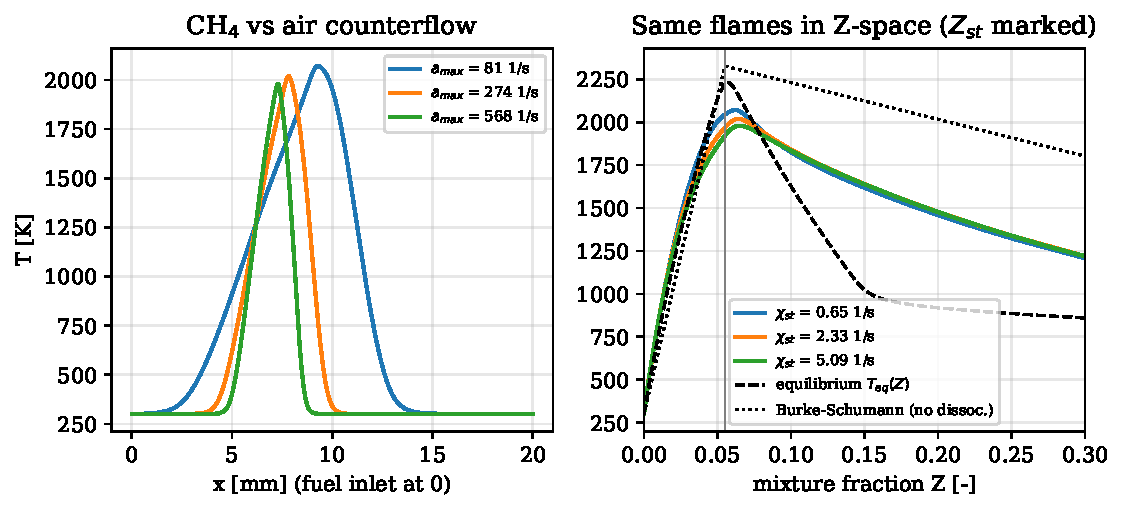
\includegraphics[width=\textwidth]{counterflow_ch4}
\caption{\ce{CH_4}/air counterflow flames at three strain rates. Left: physical space; higher strain
gives a thinner flame pushed towards the stagnation plane. Right: the same flames against Bilger $Z$,
with $T_{\rm eq}(Z)$ and Burke--Schumann. The peak temperature falls with $\chist$. On the rich side
the flames are \emph{hotter} than $T_{\rm eq}$: equilibrium would reform \ce{CH_4}+\ce{H_2O} into \ce{CO}+\ce{H_2}
(endothermic), which the flame has no time to do.}
\label{fig:cf}
\end{figure}

\section{Extinction and the S-curve}
\label{sec:scurve}

Define a Damköhler number $\mathrm{Da}=1/(\chist\tau_c)$. Plot the maximum temperature against
$\mathrm{Da}$ (or against $1/\chist$):

\begin{figure}[H]
\centering
\begin{tikzpicture}[xscale=1.6,yscale=1.1]
  \draw[->] (0,0) -- (6.4,0) node[right] {$\mathrm{Da}\propto1/\chist$};
  \draw[->] (0,0) -- (0,4.2) node[above] {$T_{\max}$};
  \draw[very thick,hot] (6,3.6) .. controls (4,3.5) and (2.4,3.2) .. (1.8,2.7);
  \draw[very thick,hot,dashed] (1.8,2.7) .. controls (1.5,2.3) and (2.2,1.6) .. (4.6,0.9);
  \draw[very thick,cold] (4.6,0.9) .. controls (4.9,0.7) and (4.8,0.5) .. (0.3,0.45);
  \draw[very thick,cold] (4.6,0.9) .. controls (5.0,0.95) and (5.5,1.05) .. (6,1.1);
  \fill (1.8,2.7) circle (2pt) node[left] {E};
  \fill (4.7,0.85) circle (2pt) node[below right] {I};
  \draw[dotted] (1.8,2.7) -- (1.8,0) node[below] {$\mathrm{Da}_E$ (extinction, $\chi_q$)};
  \draw[dotted] (4.7,0.85) -- (4.7,0) node[below] {$\mathrm{Da}_I$};
  \node[lbl,hot,align=center] at (4.6,3.85) {upper branch: burning};
  \node[lbl,align=center] at (3.6,1.85) {middle: unstable};
  \node[lbl,cold] at (2.3,0.2) {lower branch: frozen mixing};
  \draw[->,thick] (2.6,3.25) -- (1.9,2.85);
  \node[lbl] at (2.2,3.6) {increase strain};
  \draw[->,thick,warn] (1.75,2.55) -- (1.75,0.65);
\end{tikzpicture}
\caption{The S-curve. On the burning branch, increasing strain (decreasing Da) lowers $T_{\max}$
gradually until the turning point E. Beyond it no burning solution exists and the flame jumps to the
frozen branch: \textbf{extinction}. Reigniting needs the much larger Da of point I: hysteresis.}
\label{fig:scurve}
\end{figure}

\begin{figure}[H]
\centering
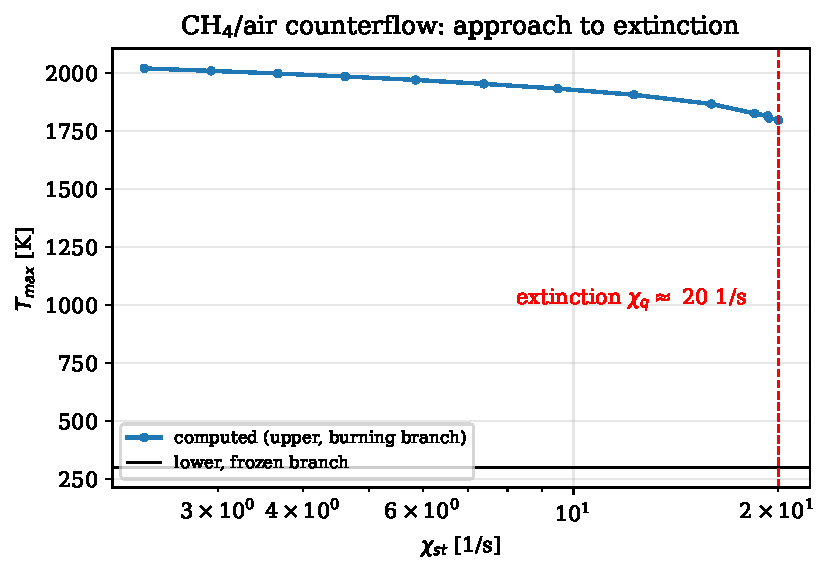
\includegraphics[width=0.85\textwidth]{extinction_ch4}
\caption{Upper branch computed with Cantera by scaling a converged \ce{CH_4}/air solution to higher strain
(and taking smaller steps whenever the next solution failed to burn). $T_{\max}$ falls slowly and then
plunges near $\chi_q$. Cantera cannot follow the unstable middle branch without special two-point
control continuation.}
\label{fig:ext}
\end{figure}

\begin{intuition}[why extinction is sudden]
As strain rises, heat leaves the reaction zone faster and $T_{\max}$ drops. Because of the Arrhenius
sensitivity (and the crossover competition for \ce{H_2}, \secref{sec:h2chain}), a modest drop in temperature
causes a large drop in reaction rate. That reduces heat release, which lowers $T$ further. Beyond a
critical point this feedback has no stable balance and the flame collapses.
\end{intuition}

\paragraph{Detecting extinction in Cantera.} After \code{solve}, check whether
$\max T$ is close to the inlet temperatures (\code{flame.extinct()} does this test), or whether the
heat release rate has vanished. A converged ``solution'' at \SI{300}{\kelvin} is a valid solution of the
equations: the frozen branch. It is not a burning flame.

\section{Why even weakly strained flames are not at equilibrium}
\begin{itemize}
  \item Finite-rate chemistry: radical recombination needs time; at any finite $\chi$ some heat is
        still stored in radicals.
  \item Differential diffusion: with $\mathrm{Le}_{\ce{H_2}}\ne1$, elements separate and the local
        enthalpy is no longer $Zh_1+(1-Z)h_2$. The local state is then not the one $T_{\rm eq}(Z)$
        assumes, and different $Z$ definitions disagree.
  \item The peak sits where reactants meet in a diffusion--reaction layer, not as a pre-mixed pocket
        given infinite time.
\end{itemize}

\begin{project}[Part 2]
\begin{itemize}
  \item Put the flame solver and $T_{\rm eq}(Z)$ in \code{ct\_utils}. Choose inlet $\dot m$ from target strains
        with the momentum-balanced formula above, then report the \emph{actual} $\chist$.
  \item Sweep strain from low to high, restarting each solve from the previous solution. When a solve
        lands on the frozen branch, you have bracketed extinction.
  \item Questions: asymmetry (the two reasons in the intuition box); peak shift with $\chist$ (look at
        where $T_{\max}$ sits relative to $\Zst$ as $\chi$ grows); the area between $T(Z)$ and $T_{\rm eq}(Z)$
        (energy not yet released: finite-rate plus differential diffusion); extinction detection (above).
\end{itemize}
\end{project}

\begin{selfcheck}
\begin{enumerate}
  \item Compute $\Zst$ for \ce{H_2}/air by hand. Where, relative to the stagnation plane, will the flame sit?
  \item If you double the strain rate, by what factor does $\chist$ change according to \eqref{eq:chiZ}?
        And the flame thickness $\ell$?
  \item Why does the frozen branch of the S-curve satisfy the steady counterflow equations?
\end{enumerate}
\end{selfcheck}
